% \documentclass[tikz]{standalone}
% \usepackage{tikz}
% \usepackage{pgfplots}
% \pgfplotsset{compat=1.18}

% \begin{document}
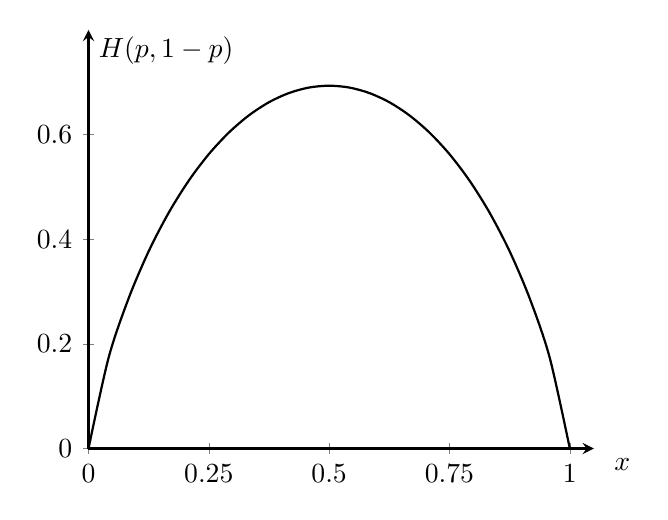
\begin{tikzpicture}
    \pgfplotsset{
    width=8cm,
    every axis/.append style={thick},
    }
    \begin{axis}[
        ymin=0, ymax=0.8,
        xmin=0, xmax=1.05,
        axis x line=left,
	    axis y line=left,
        legend style={draw=none},
        xtick={0,0.25,0.5,0.75,1},
        ytick={0,0.2,0.4,0.6},
        legend pos=south east,
        every axis x label/.style={
            at={(ticklabel* cs:1.02)},
            anchor=north west,
        },
        every axis y label/.style={
            at={(ticklabel* cs:0.95)},
            anchor=west,
        },
        label style={font=\normalfont},
        xlabel={$x$},ylabel={$H(p,1-p)$}
    ]
    \addplot[domain =0:1, smooth] {-x*ln(x)-(1-x)*ln(1-x)};
    \end{axis}
    \end{tikzpicture}
% \end{document}